% !TeX program = xelatex
\documentclass[catalan]{beamer}
\newcommand{\intRutaPaquete}{../}
\usepackage[tikz]{../jma}

\title{Prova de les eines bàsiques}
\author{Joaquín Millán Aldaz}


\begin{document}
\begin{frame}
	\titlepage
	\url{https://github.com/jma25l/tex-jma}
\end{frame}
\begin{frame}
	\centering
	%\titulo
	\textbf{HOLA}\\
	\[\N \subset \Z \subset \Q \subset \R \subset \C \]
	\[\mathbb E(k) = \mathbb E(k\ind_\Omega) = k\]
	\[
		\begin{array}{ccc}
		\text{Subespais projectius } P(E) & \biy & \text{Subespais vectorials }E\\
		{\color{blue} \biyV} & & \biyV\\ 
			\text{Subespais projectius } P(E^{*}) & \biy & \text{Subespais vectorials }E^{*}\\
		\end{array}
	\]
\end{frame}
\begin{frame}
	\textbf{Proposició: }\\
	Un graf és eulerià si i només si com a màxim hi ha dos vèrtexs de grau senar. 
	\directa
	Tinc un recorregut eulerià, que passa només una vegada per cada aresta. Excloent-ne els dos vèrtexs dels extrems, [...]
	\reciproc
	[...] 
	\qed
\end{frame}
\begin{frame}
	\centering
	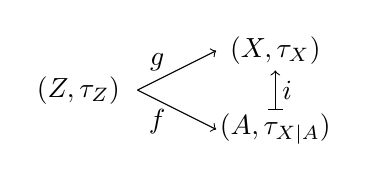
\begin{tikzpicture}
    \node at (-1.25, 0) {$(Z, \tau_Z)$};
    \node at (1.25, 0.5) {$(X, \tau_{X})$};
    \node at (1.25,-0.5) {$(A, \tau_{X|A})$};
    
    \draw[->] (-0.5, -0) -- (0.5, -0.5);
    \draw[->] (-0.5, -0) -- (0.5, 0.5);
    \draw[|->] (1.25, -0.25) -- (1.25, 0.25);
    \node at (-0.25, 0.35) {$g$};
    \node at (-0.25, -0.40) {$f$};
    \node at (1.40, 0) {$i$};
\end{tikzpicture}
\end{frame}
\end{document}